\documentclass{scrartcl}
\usepackage[UKenglish]{babel}
\usepackage{graphicx}

\usepackage{caption}
\usepackage{subcaption}

\usepackage{hyperref}

\usepackage{cleveref}

\title{Advanced Data Analysis and Machine Learning - Practical Activities}
\subtitle{Sequential Data}
\author{Sergio Mauricio Vanegas Arias}
\date{\today}

\begin{document}

\maketitle

\section{Introduction}

  This week, we were asked to experiment with sequential data, both from a time-series dataset on water quality and an arbitrary text file, applying the data processing techniques reviewed in class.

  For the time series, we were asked to perform seasonality analysis, first through \textit{Seasonal-Trend decomposition using LOESS}, and then through univariate and multivariate K-means clustering. Finally, we were asked to propose a dataset partition strategy based on the obtained results.

  For the text data, we were asked to plan and execute a pre-processing algorithm on a text file of our choice. Then, we were asked to visualize the clean dataset using 3 different representations. Finally, we were requested to devise a strategy for segmenting the text data into sub-sequences, ready
  to be fed to a neural network.

\section{Environmental Time Series}

  The first step was to perform an automatic decomposition on the dataset signals. The results for the first input variable and the water quality signal are shown in \Cref{fig:STL_auto}.

  \begin{figure}[ht]
    \centering
    \begin{subfigure}[b]{0.8\textwidth}
      \centering
      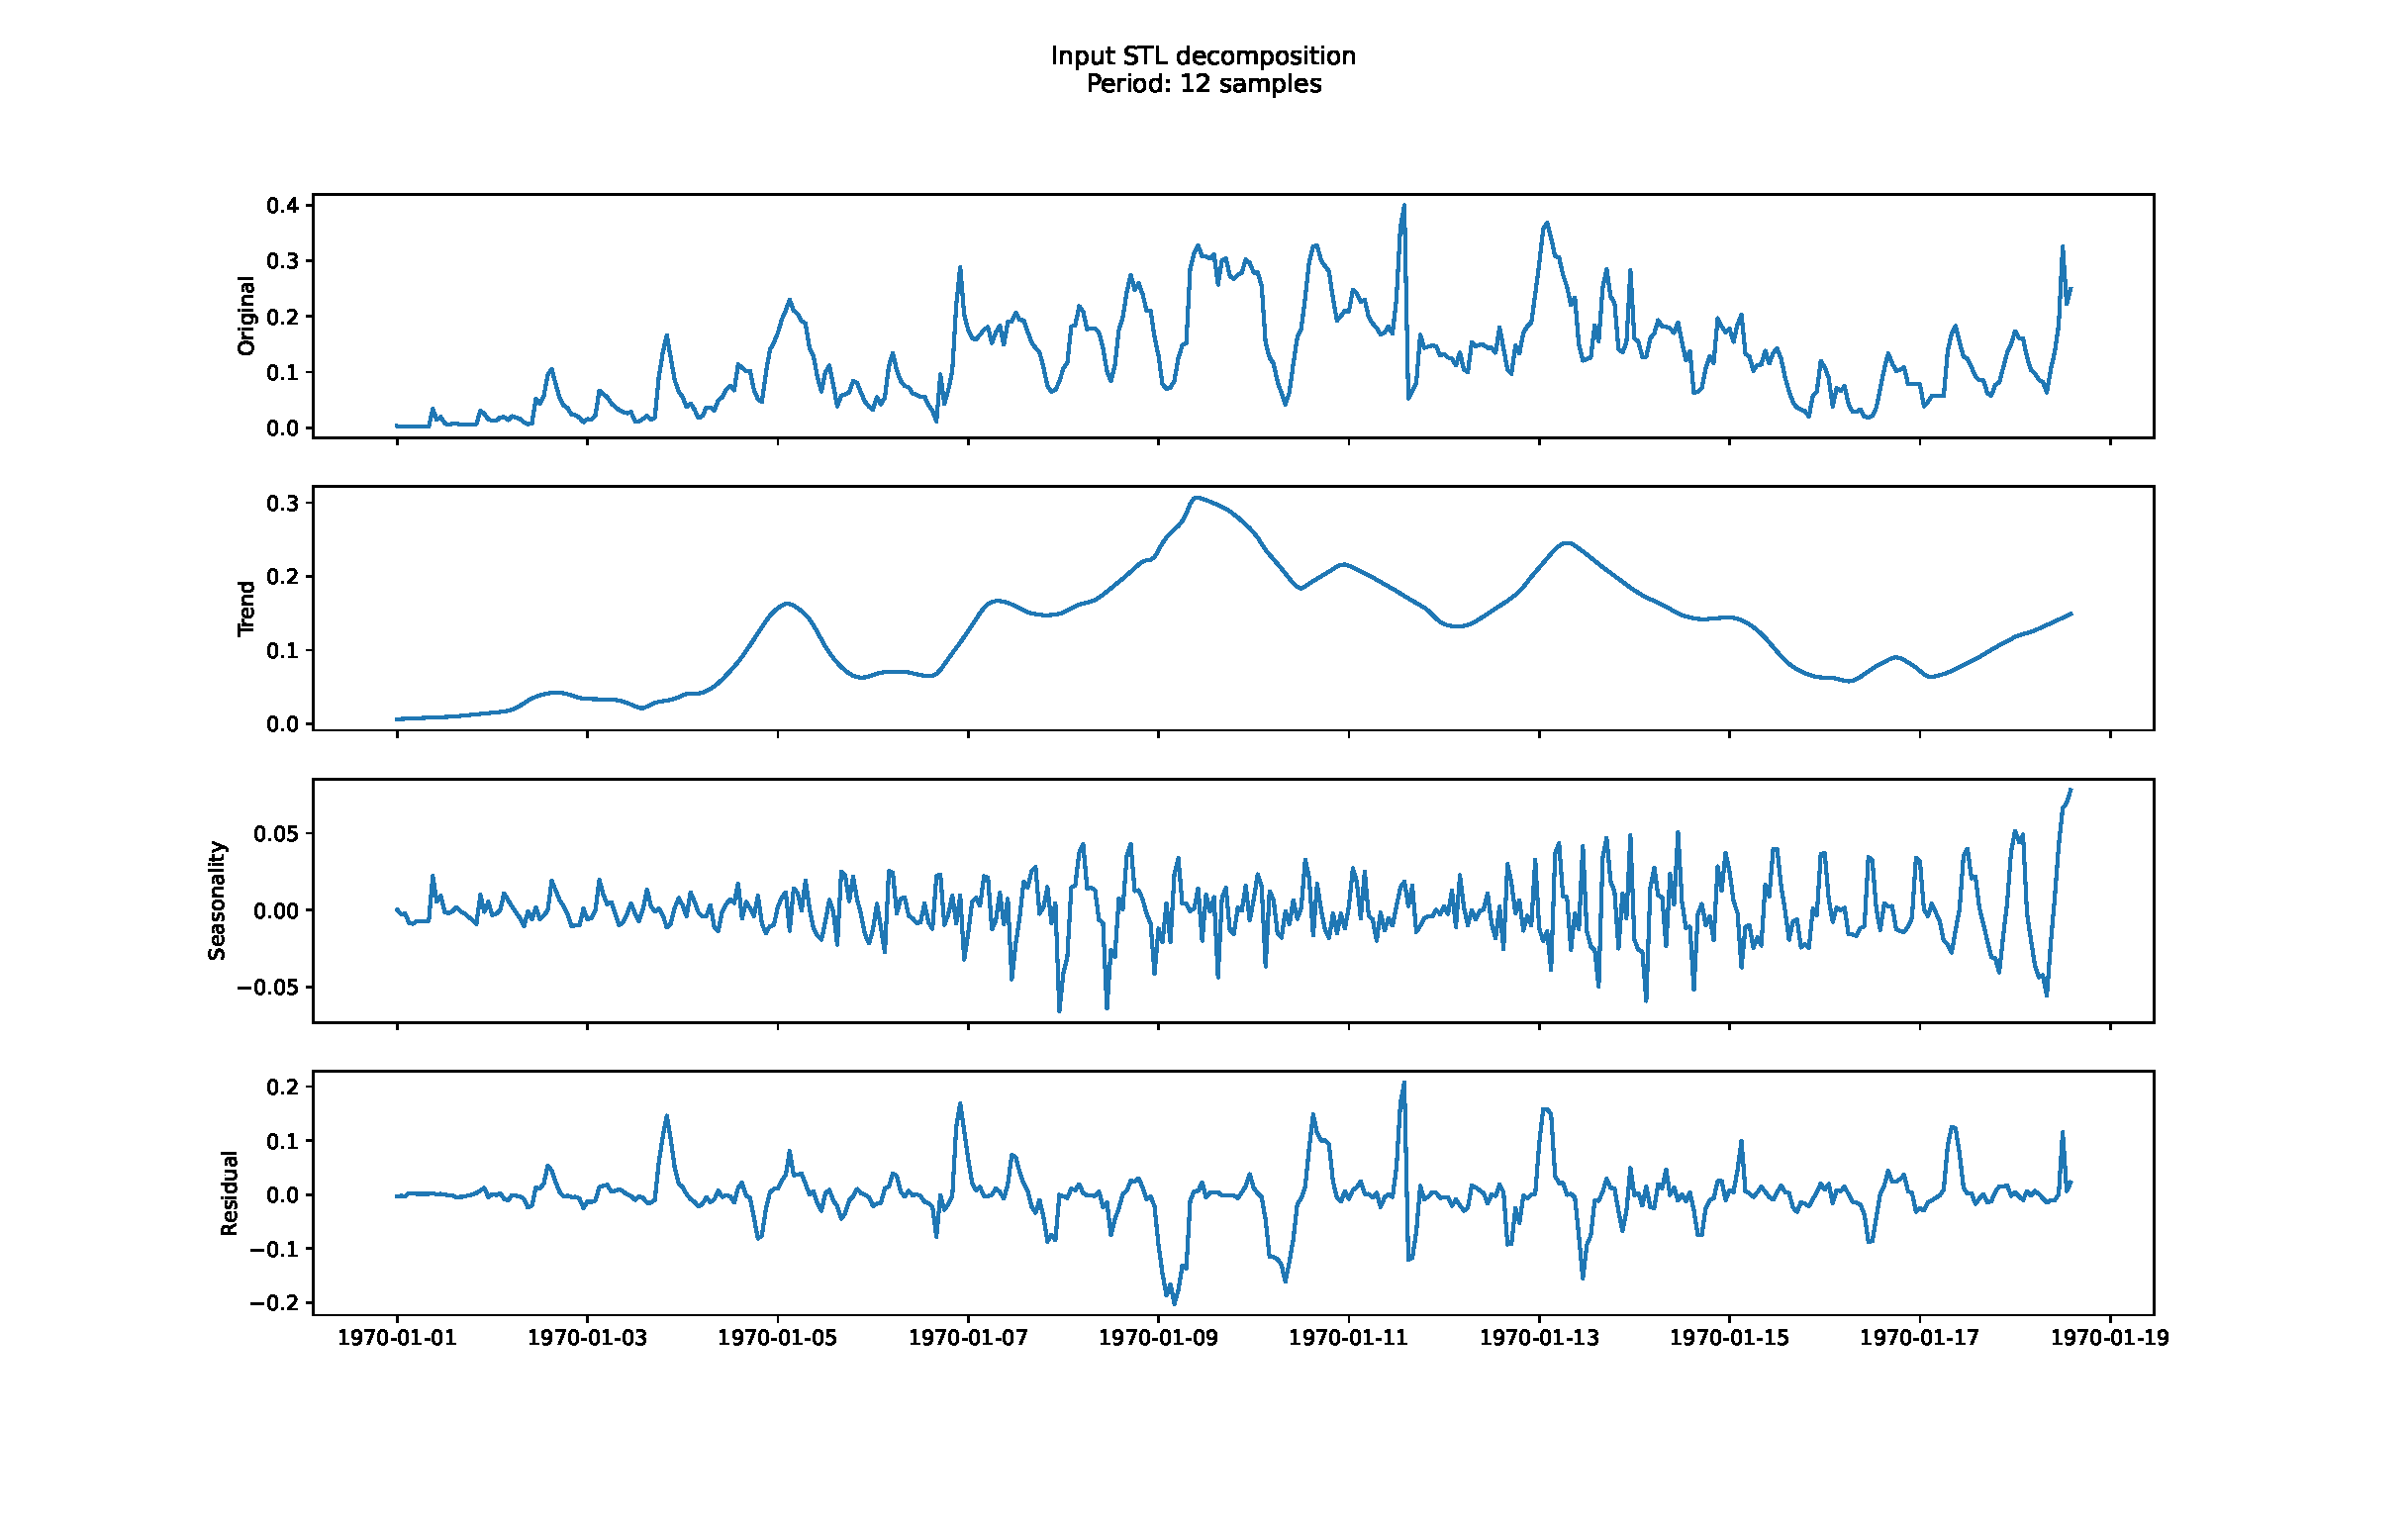
\includegraphics[width=\textwidth]{./figures/x_decomp.eps}
      \caption{Input signal decomposition}
      \label{fig:x_decomp}
    \end{subfigure}
    \hfill
    \begin{subfigure}[b]{0.8\textwidth}
      \centering
      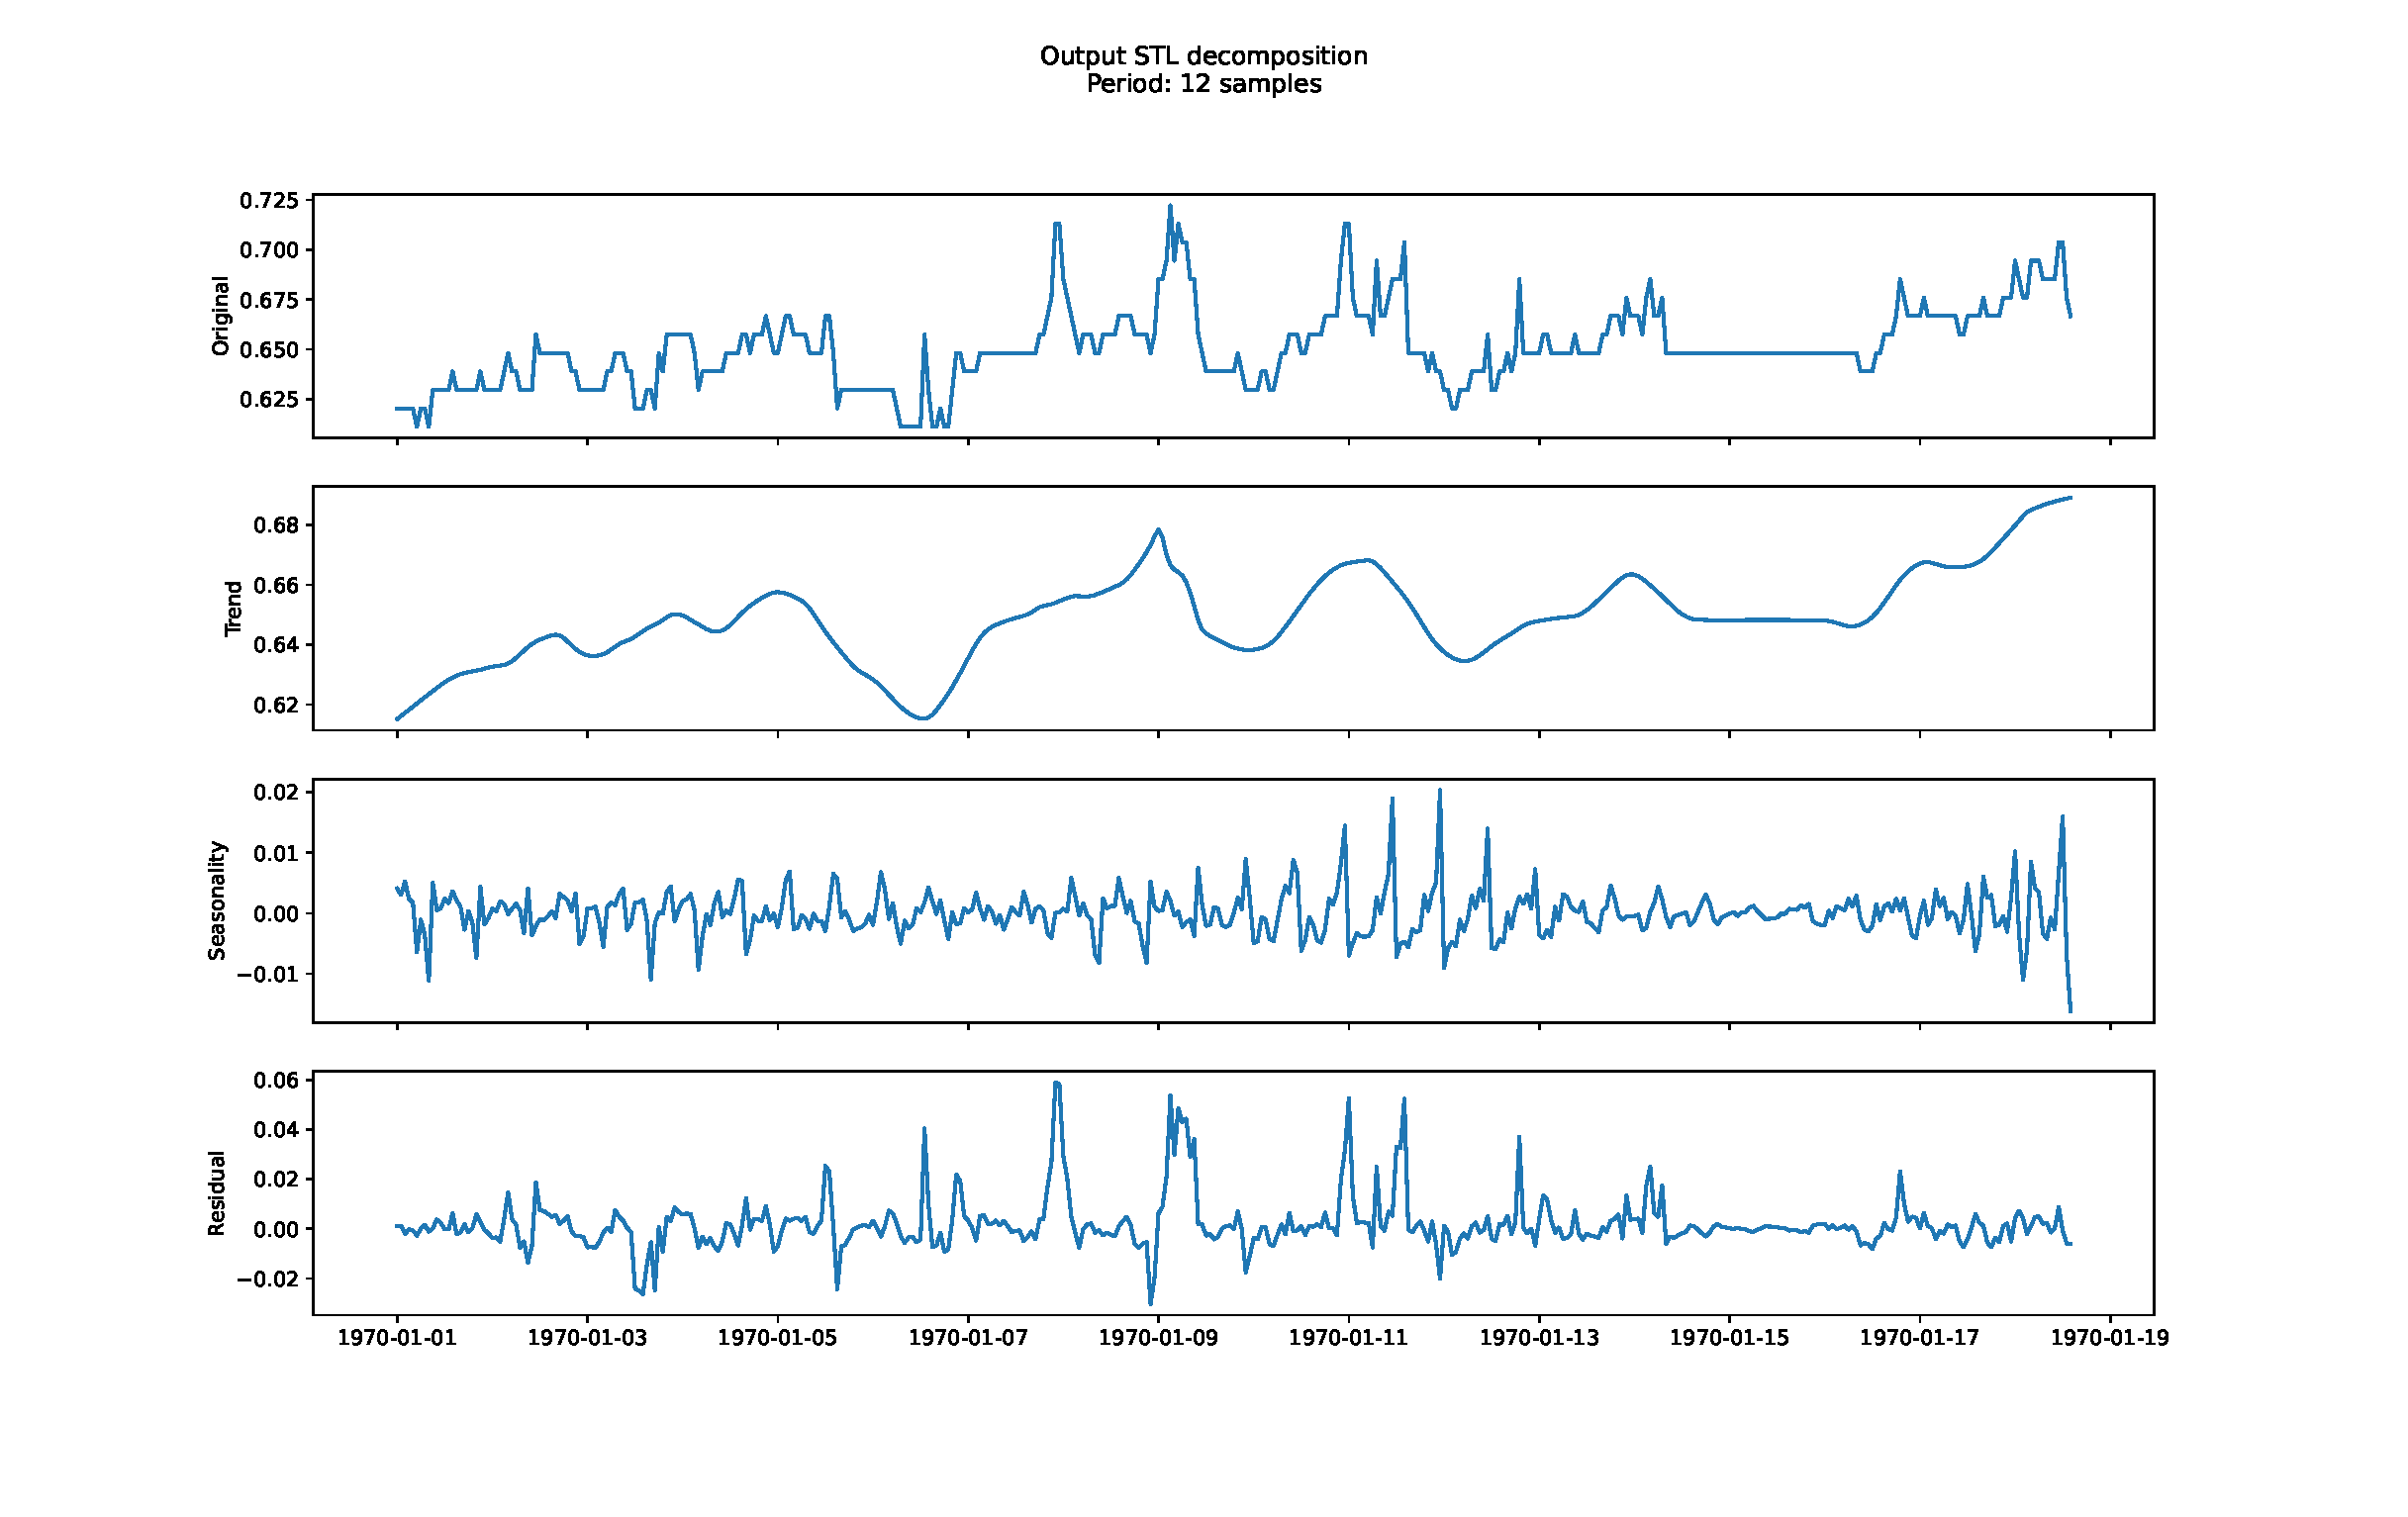
\includegraphics[width=\textwidth]{./figures/y_decomp.eps}
      \caption{Output signal decomposition}
      \label{fig:y_decomp}
    \end{subfigure}
    \caption{Automatic STL decomposition}
    \label{fig:STL_auto}
  \end{figure}

  Despite the algorithm's best efforts to identify the periodicity of the signals, the results end up being rather underwhelming: the trend component ends up absorbing most of the signal's shape, with the seasonality component lacking any representativeness of the original behaviour. Thus, a manual imputation of the signal's period is performed.

  \begin{figure}[ht]
    \centering
    \begin{subfigure}[b]{0.65\textwidth}
      \centering
      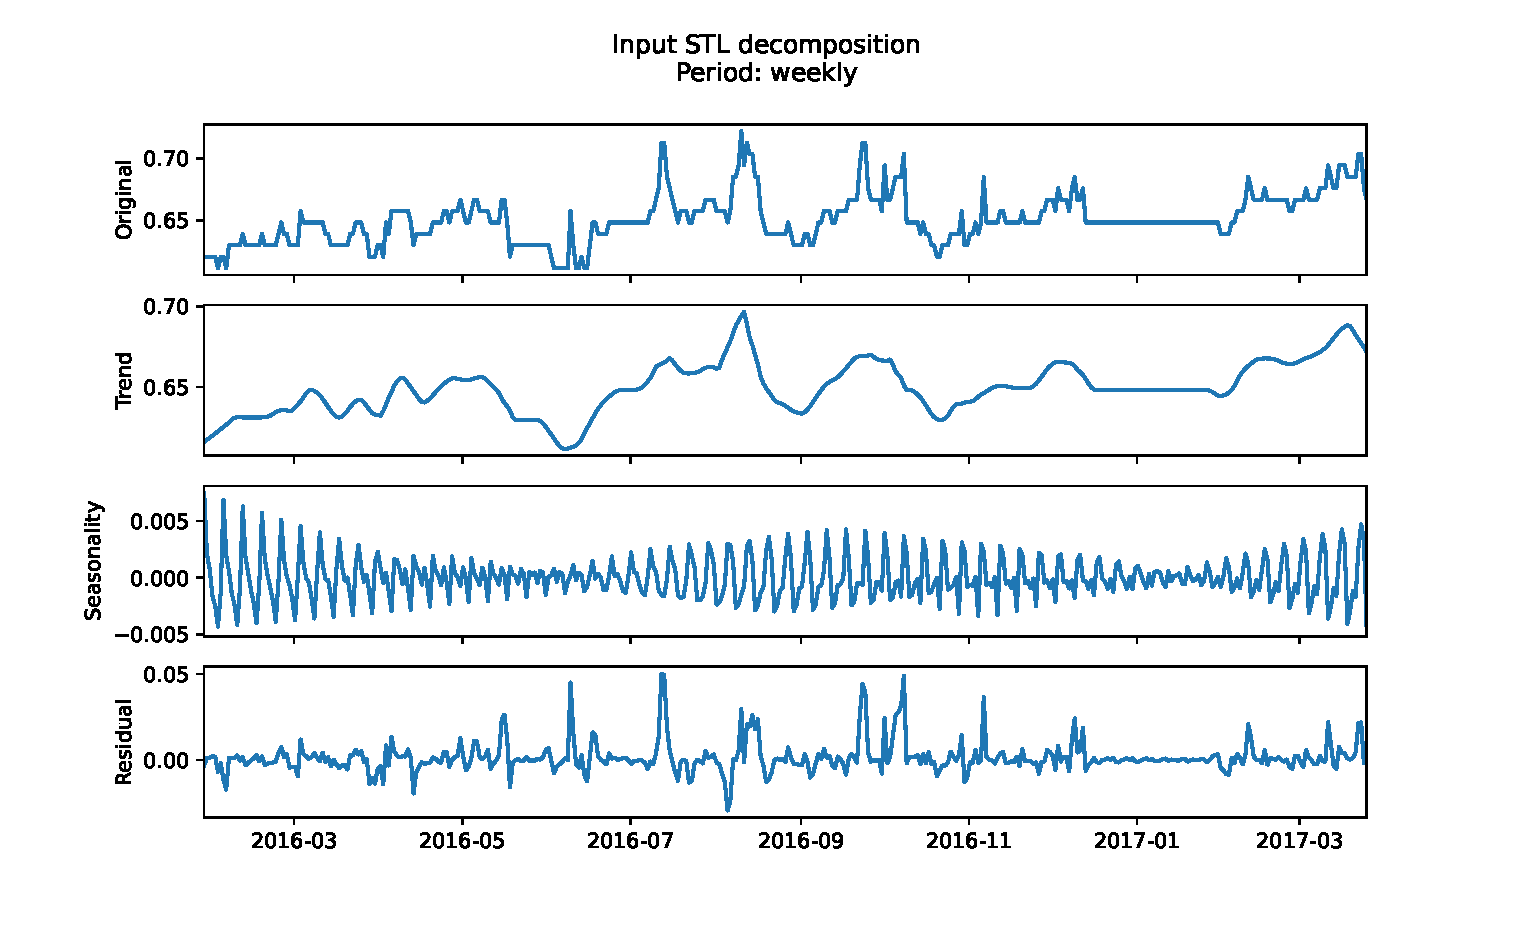
\includegraphics[width=\textwidth]{./figures/weekly_decomp.eps}
      \caption{Input signal decomposition}
      \label{fig:weekly_decomp}
    \end{subfigure}
    \hfill
    \begin{subfigure}[b]{0.65\textwidth}
      \centering
      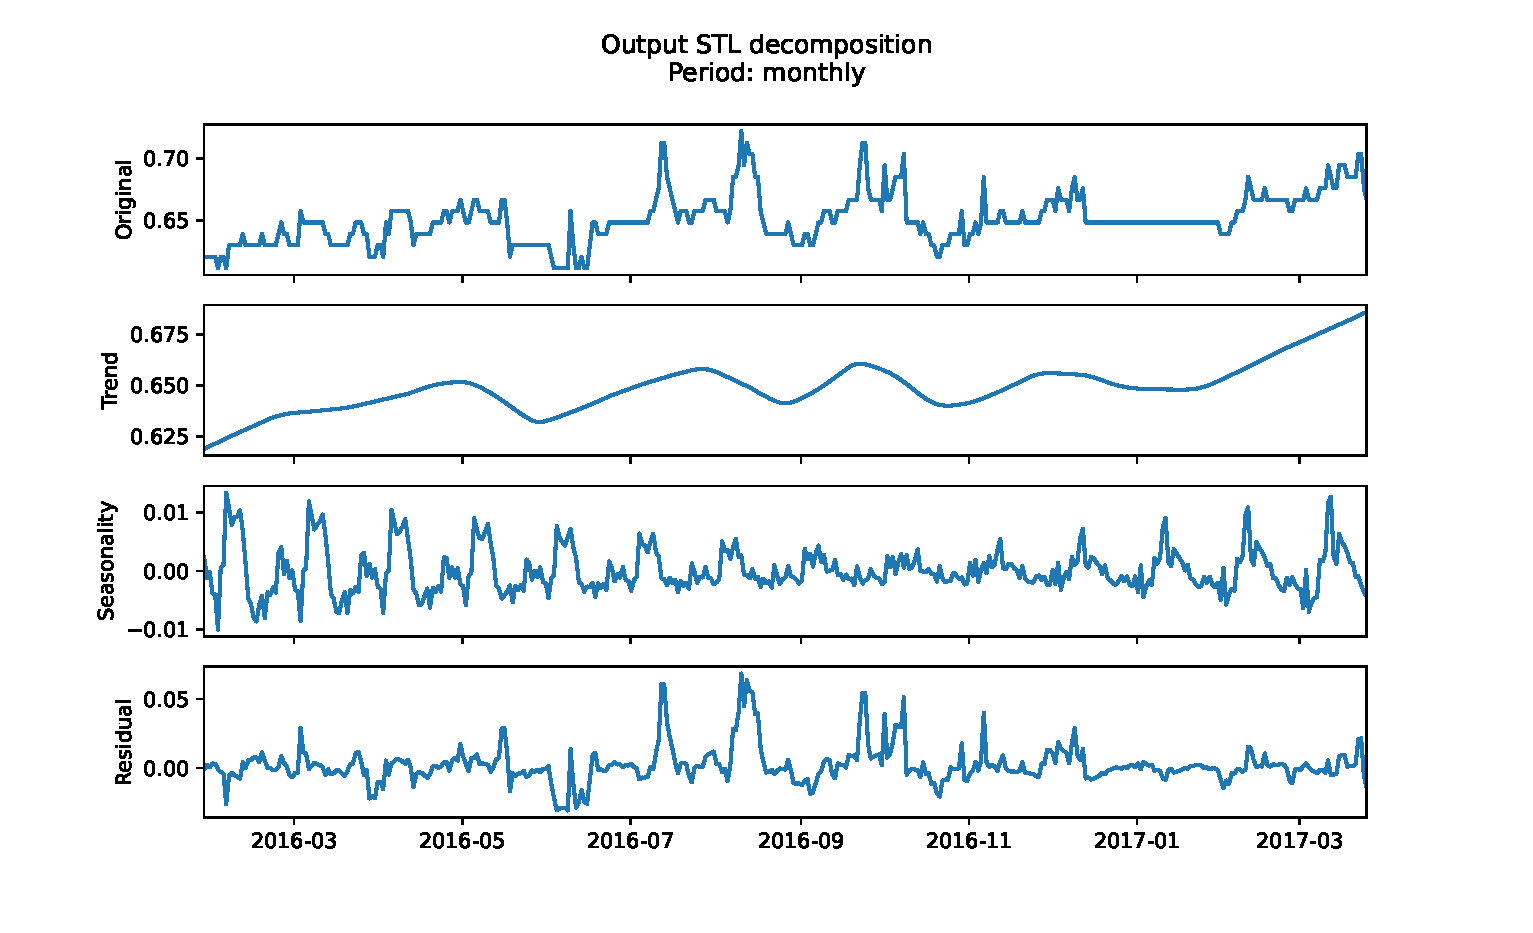
\includegraphics[width=\textwidth]{./figures/monthly_decomp.eps}
      \caption{Output signal decomposition - monthly periodicity}
      \label{fig:monthly_decomp}
    \end{subfigure}
    \hfill
    \begin{subfigure}[b]{0.65\textwidth}
      \centering
      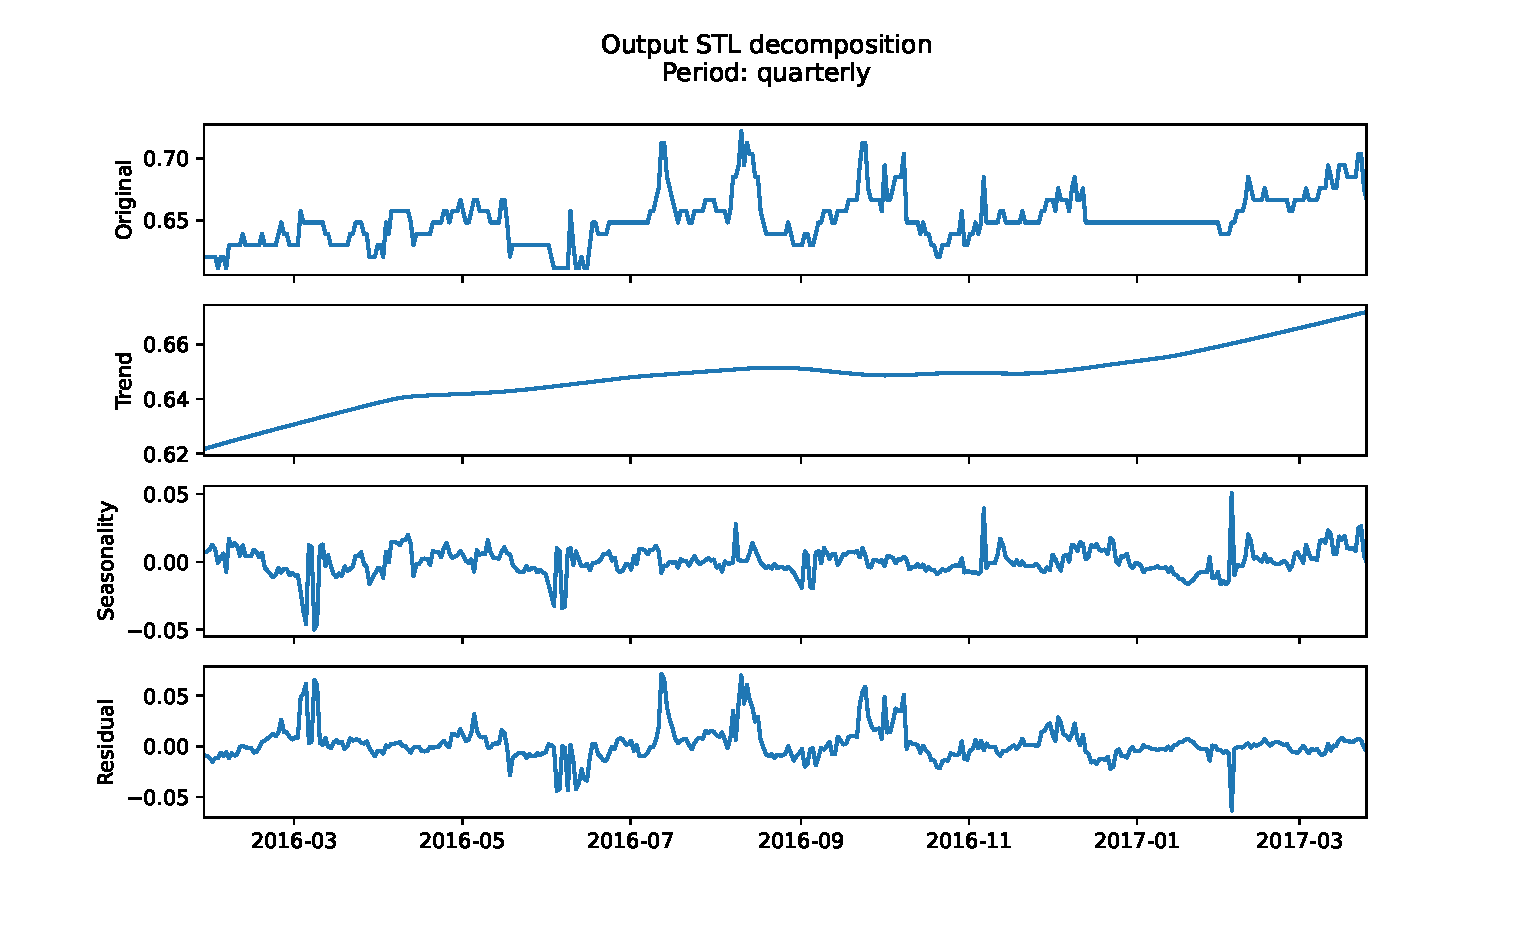
\includegraphics[width=\textwidth]{./figures/quarterly_decomp.eps}
      \caption{Output signal decomposition - quarterly periodicity}
      \label{fig:quarterly_decomp}
    \end{subfigure}
    \caption{Manual STL decomposition}
    \label{fig:STL_manual}
  \end{figure}

  In \Cref{fig:STL_manual}, the STL decompositions for weekly, monthly, and quarterly periodicity are displayed. In \Cref{fig:weekly_decomp}, we can observe the same issue as in \Cref{fig:y_decomp}, which implies this might have been the automatically detected periodicity value; just as above, the magnitude of the seasonality component ends up being so low that it gets overwhelmed by the residual component, rendering the decomposition useless.

  On the other hand, both \Cref{fig:monthly_decomp,fig:quarterly_decomp} manage to display a repeating pattern on the water quality variable; particularly, the quarterly decomposition is able to do this without preserving regular oscillations in the trend component, which is congruent with its definition. With these results in mind, a K-means approach followed.

  \begin{figure}[ht]
    \centering
    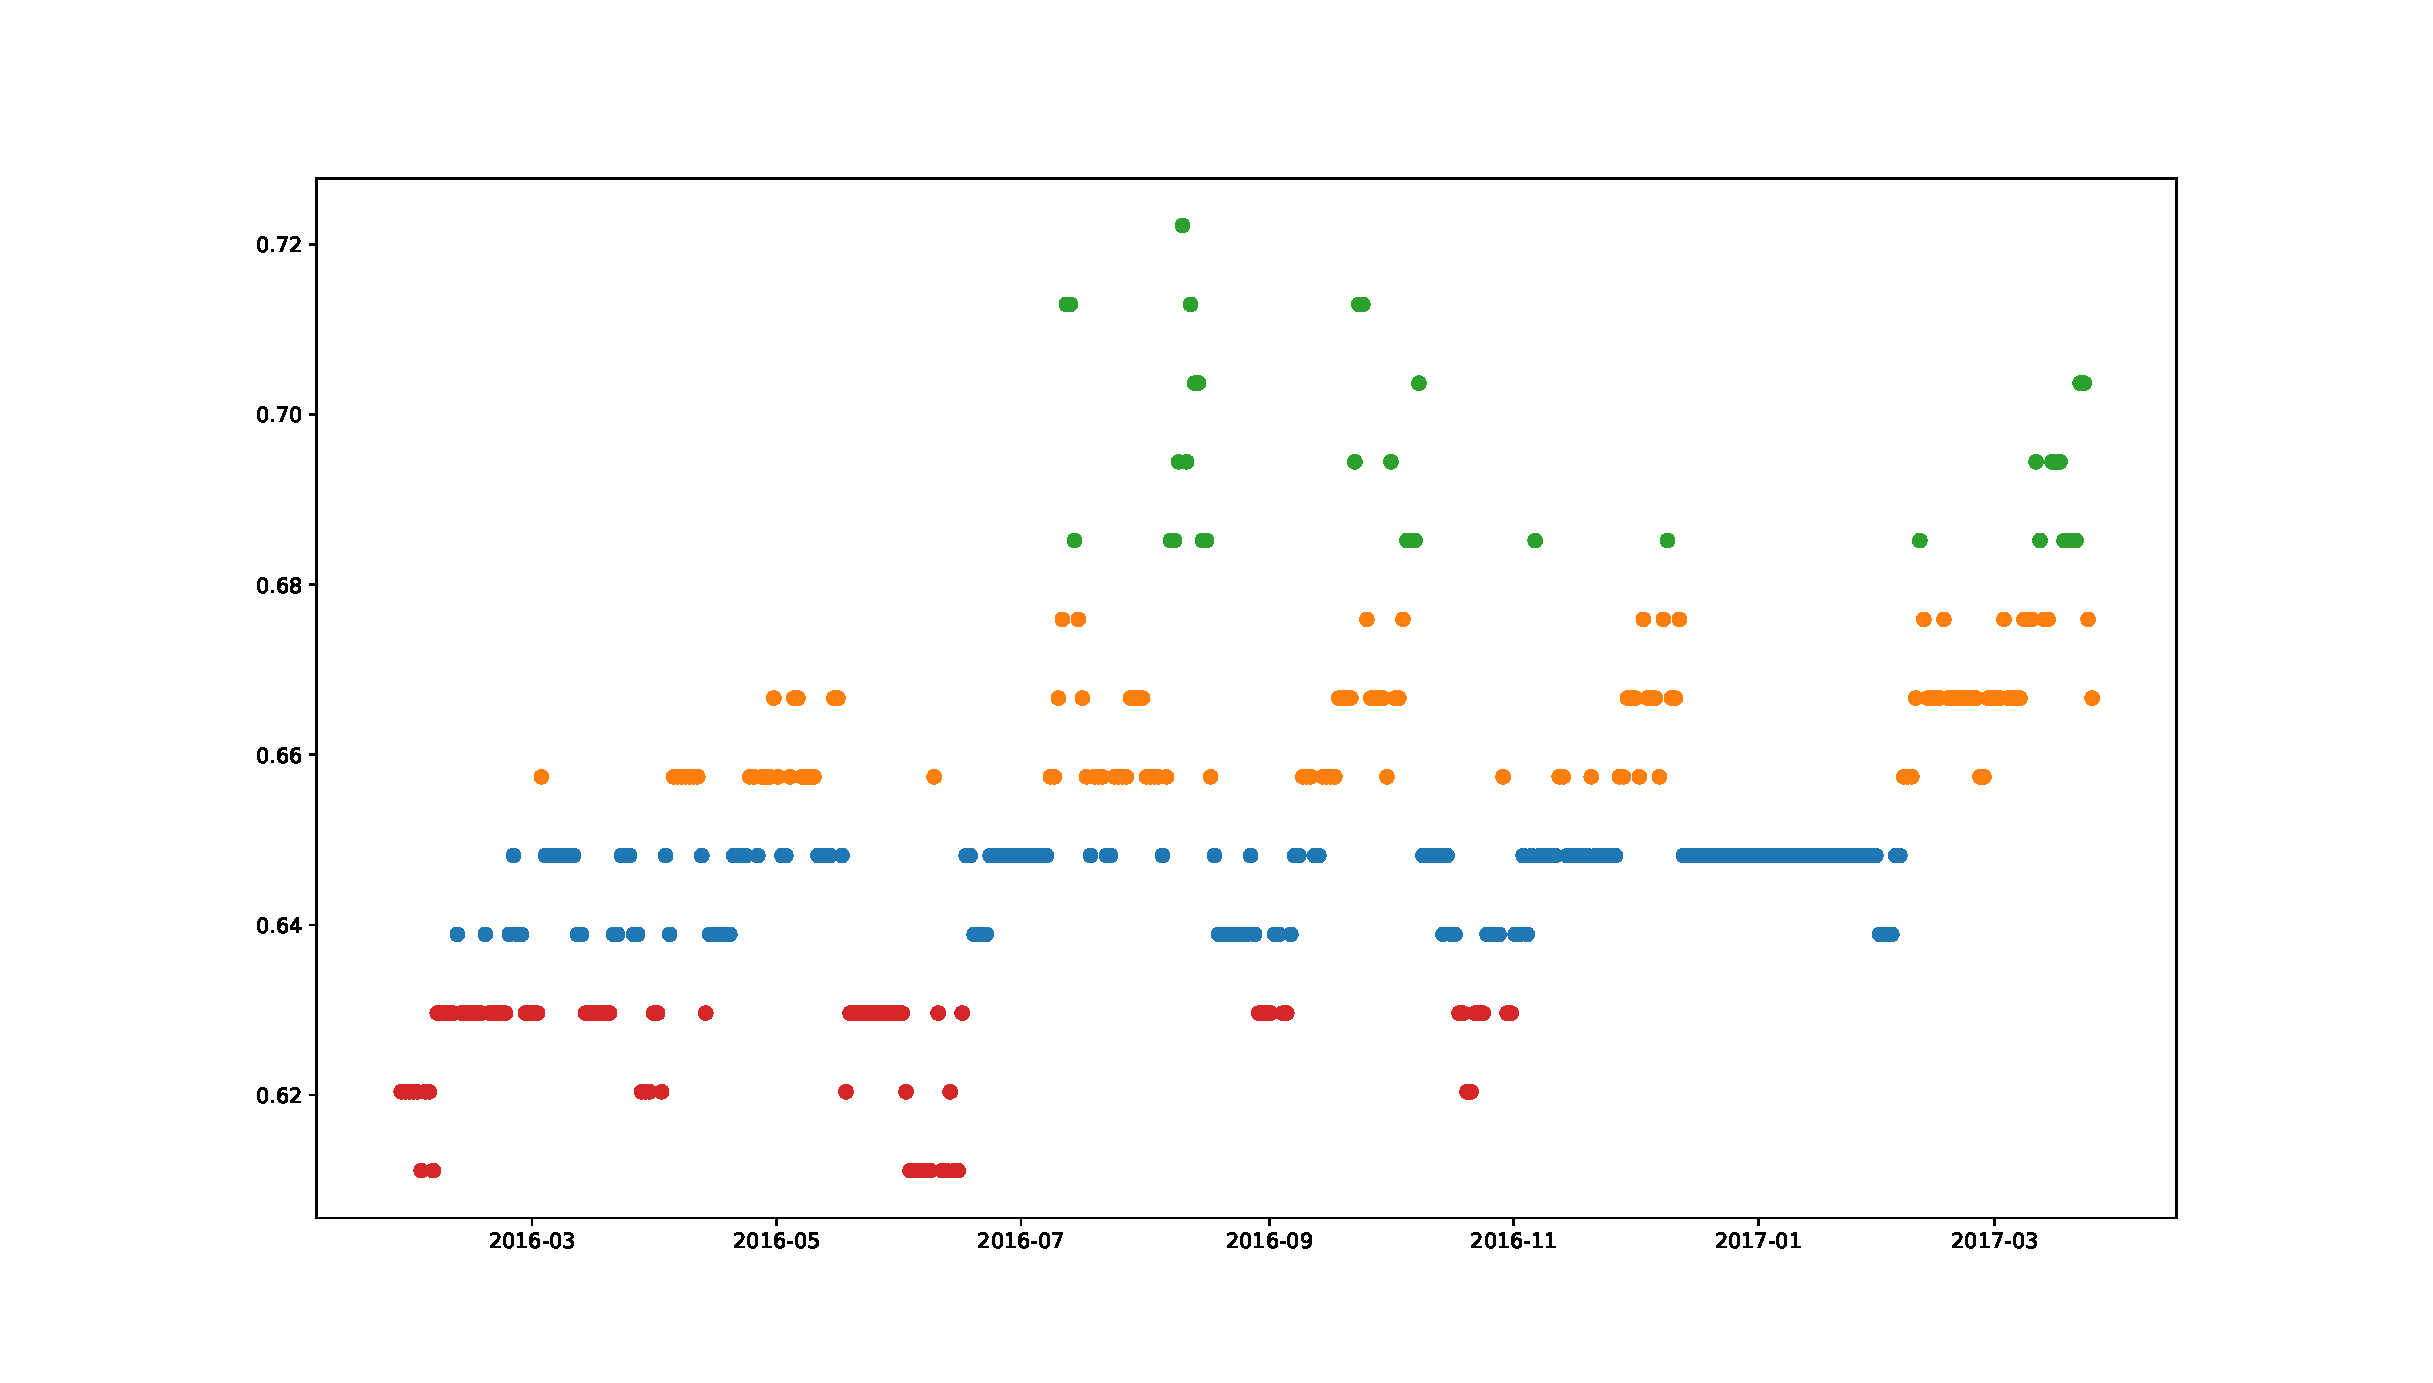
\includegraphics[width=0.8\textwidth]{./figures/clustered_by_output.eps}
    \caption{Univariate clustering}
    \label{fig:univariate_clustering}
  \end{figure}

  In \Cref{fig:univariate_clustering}, a 4-cluster K-Means classification of the time series based exclusively on the \textit{water quality} variable is applied. As expected, the algorithm only separates the samples based on their magnitude, so no information on seasonality can be derived from this approach.

  \begin{figure}[ht]
    \centering
    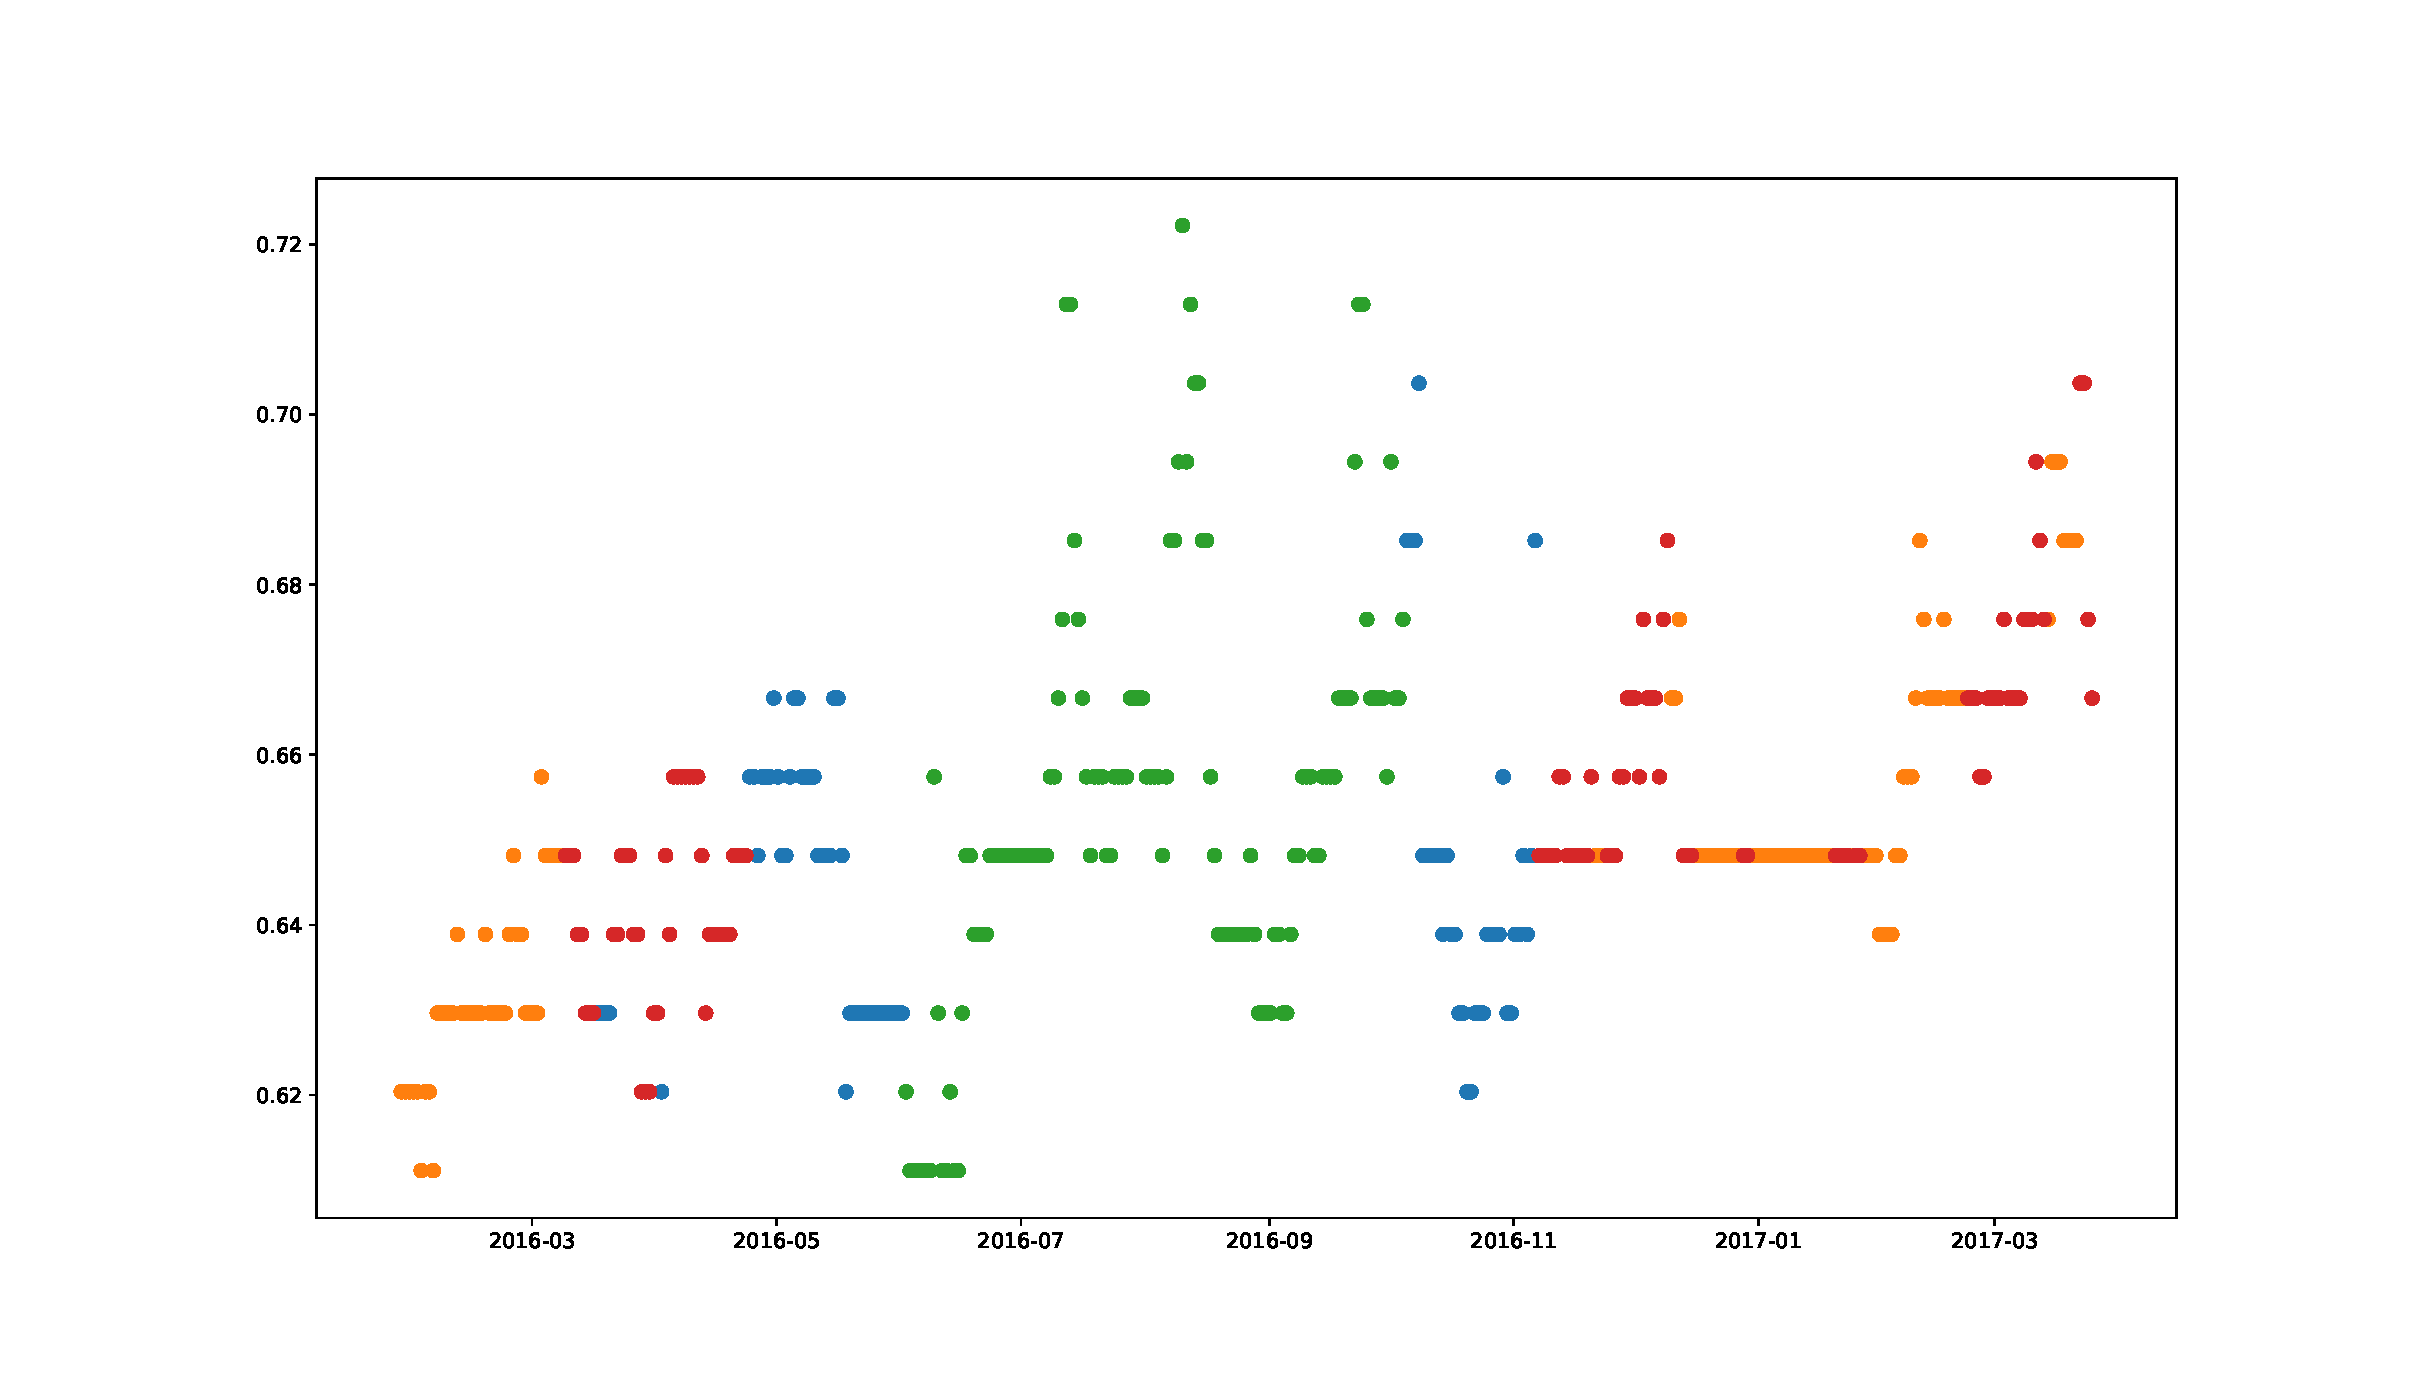
\includegraphics[width=0.8\textwidth]{./figures/clustered_by_input.eps}
    \caption{Multivariate clustering}
    \label{fig:multivariate_clustering}
  \end{figure}

  On the other hand, in \Cref{fig:multivariate_clustering} we can observe a clear separation of some critical regions, particularly in the middle section of the signal and the transition regions around it. The cluster overlap near the ends of the signal seem to indicate a cyclical behaviour, which is consistent with the results of the STL analysis.

  Based on these results, the following partition strategy would be suggested:

  \begin{itemize}
    \item Partition the entire dataset intro quarters.
    \item For each quarter, reserve the first fraction of the time-series for testing and use the rest of the trimester for training in order to avoid causality bias and help with generalization.
    \begin{itemize}
      \item Alternatively, the earliest and latest samples of each quarter can also be used for training in order to help the model learn the dynamics of the transition, with the middle section being used for validation instead.
    \end{itemize}
  \end{itemize}

\section{Sequential Text Data}

  For this section, the short story \href{https://www.hplovecraft.com/writings/texts/fiction/d.aspx}{\textit{Dagon}} by author \textit{Howard Phillips Lovecraft} was selected.

  Normally, a pre-processing pipeline for sequential text data would consist of the following steps:

  \begin{enumerate}
    \item De-capitalise the text; i.e., convert all upper-case letters into lower-case.
    \item Remove URLs
    \begin{itemize}
      \item Not necessary in this case, since we're dealing with a literary text.
    \end{itemize}
    \item Remove punctuations, digits, and special symbols.
    \item Tokenize the text string, splitting it by white-spaces/newlines.
    \item Remove common \textit{stop-words} by comparing the tokenized text to a pre-existent collection.
    \item ``Normalize'' the words by applying a stemming or lemmatization algorithm.
    \begin{itemize}
      \item Given the ``age'' of the text, the available stemming algorithms proved to be inaccurate, so this step had to be skipped.
    \end{itemize}
  \end{enumerate}

  Fortunately, the \href{https://amueller.github.io/word_cloud/}{\textit{wordcloud}} module for Python already implements most of these steps, so the only deviation from the suggested pipeline was extending the list of stop-words with the collection in the \href{https://www.nltk.org/}{NLTK} module. The word cloud for the cleared vocabulary is shown in \Cref{fig:wordcloud}, whereas the bigram and trigram are displayed in \Cref{fig:N_gram}.

  \begin{figure}[ht]
    \centering
    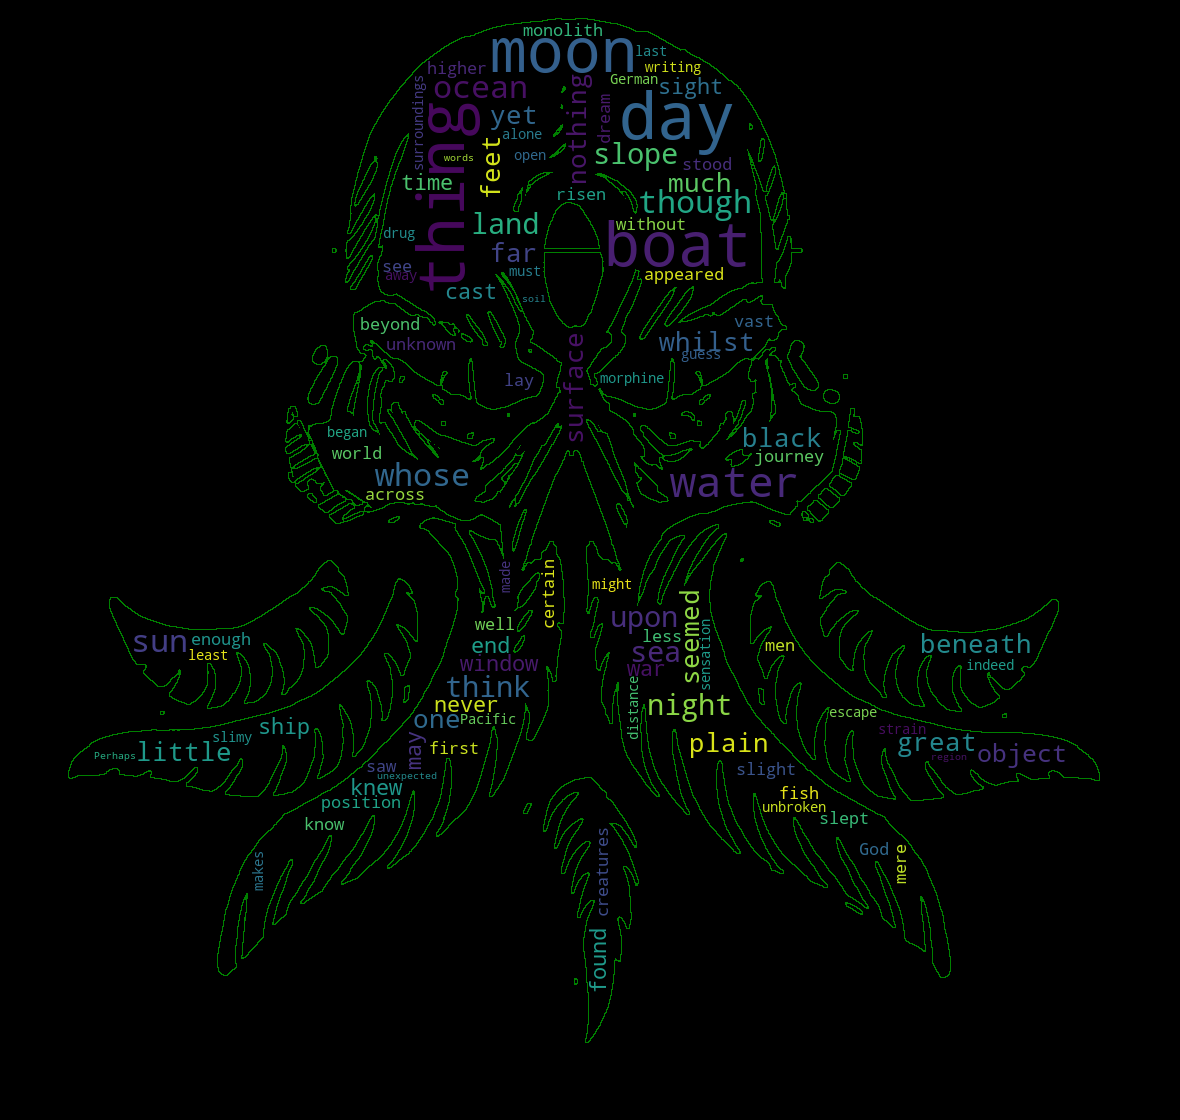
\includegraphics[width=0.8\textwidth]{./figures/wordcloud.png}
    \caption{Cleared-vocabulary word cloud}
    \label{fig:wordcloud}
  \end{figure}

  \begin{figure}[ht]
    \centering
    \begin{subfigure}[b]{0.49\textwidth}
      \centering
      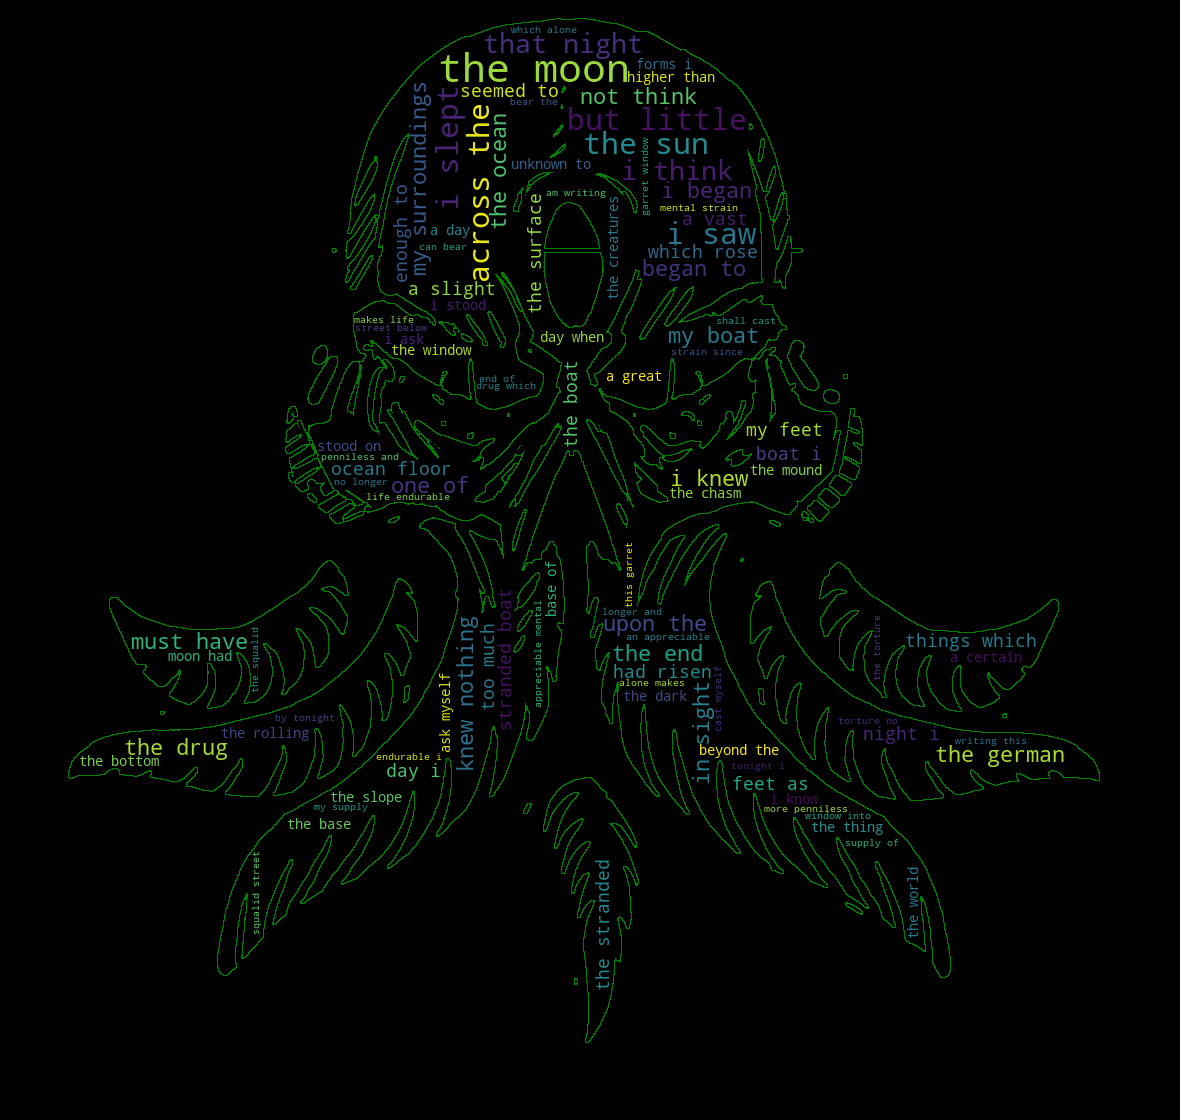
\includegraphics[width=\textwidth]{./figures/wordcloud_2N.png}
      \caption{bigram word cloud}
      \label{fig:bigram}
    \end{subfigure}
    \hfill
    \begin{subfigure}[b]{0.49\textwidth}
      \centering
      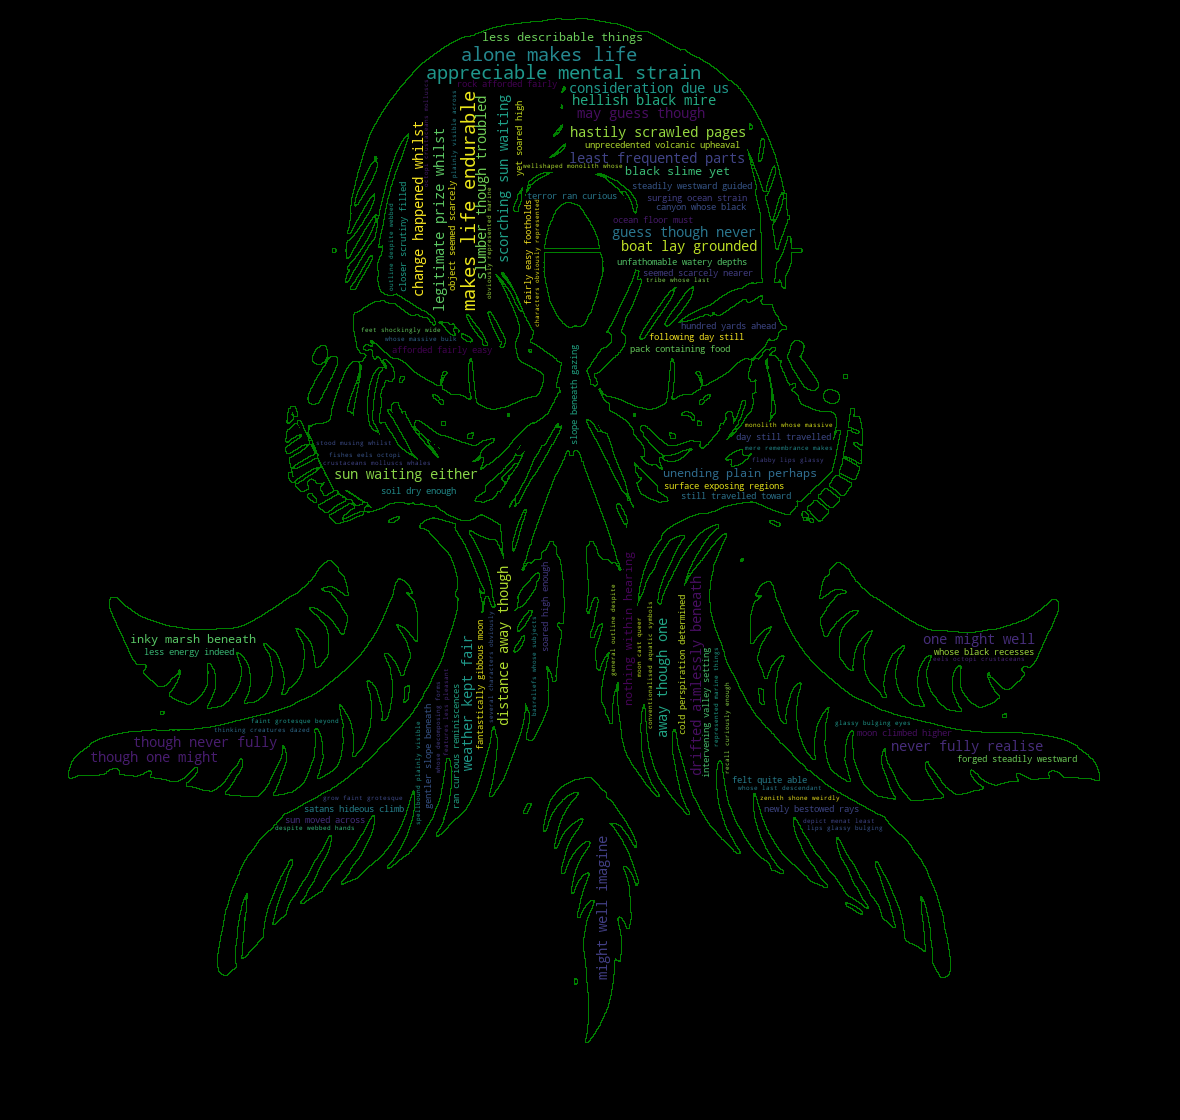
\includegraphics[width=\textwidth]{./figures/wordcloud_3N.png}
      \caption{trigram word cloud}
      \label{fig:trigram}
    \end{subfigure}
    \caption{N-gram word clouds}
    \label{fig:N_gram}
  \end{figure}

  Regarding the data segmentation strategy: modern LLMs based on the \href{https://en.wikipedia.org/wiki/Transformer_(machine_learning_model)}{Transformer Architecture} organize tokenized N-grams into look-up tables and train their coefficients based on the desired next token, making use of a \textit{Softmax} output layer to return the token with the highest probability of being the correct one. In our case, however, a different strategy is required, since the target is to predict the next letter instead of the next word. One option would be to set the input size of the model to the length of the longest word in English (\textit{pneumonoultramicroscopicsilicovolcanoconiosis}, with 45 characters), and then tokenize individual characters (including white-spaces and apostrophes, but ignoring other special characters), assigning a numerical value to each of them. An example of input/output for predicting the last character in the text sequence \textit{``The quick brown fox jumps over the lazy dog''} would be:

  \begin{center}
    \begin{tabular}{| c c c c c c c c || c |}
      $x[1]$ & $x[2]$ & $x[3]$ & $x[4]$ & $x[5]$ & $\dots$ & $x[44]$ & $x[45]$ & $y$ \\
      \hline
      $\_$ & $\_$ & $\_$ & T & h & $\dots$ & d & o & g 
    \end{tabular}
  \end{center}

  Of course, a network architecture capable of preserving context beyond immediate input is also required for this approach to work adequately.

\end{document}